% Hier steht der Rezepttitel
\section{Lasagne}
% Untertitel
\large{Effort that entails success!}
\begin{centering}
% Danach die Zutaten in Tabellenform
% Wie viele werden satt?
Serves 6 hungry eaters
\end{centering}
%\textbf{Zutaten:}
\begin{table}[H]
  \centering
    % eine Tabelle mit insgesamt 4 Spalten, falls mehr Zutaten benoetigt werden
    % links: Menge, rechts: Zutat
  \begin{tabular*}{1\textwidth}{rlrl}
    &\textbf{Ragu Bolognese:}&&\\
    %&  &&  \\
    1 & carrot & 1 stick & celery \\
    1.8\,oz  & Pancetta & 1 & onion \\
    2 cloves of & garlic &1\,tbs & butter\\
    1\,tbs & olive oil & 10.5\,oz&mixed minced meat\\
    1.7\,cups/14\,oz (400\,g)&peeled tomatoes&1.25\,cups/10\,oz& red wine/vegetable broth\\
    &salt & & black pepper\\
    &&&\\

    &\textbf{Sauce Bechamel:}&&\\
    1.8\,oz & butter & 1.8\,oz & flour \\
    3.2\,cups & milk & & salt \\
    &black pepper& & ground nutmeg\\
    &&&\\
    &\textbf{To build layers:}&&\\
    8.8\,oz & pasta  & & salt\\
    8.8\,oz & mozzarella & 3.5\,oz & freshly grounded parmesan\\
    1\,tbs & butter
  \end{tabular*}
\end{table}

%Zubereitung:
\begin{Notes}
  \item For the bolognese peel the carrots and wash celery, cut into fine
    dice. (The bolognese is the same as for the spaghetti sauce). Proceed with
    the pancetta likewise and also with the garlic and the onion after having
    them peeled.
    
  \item Heat butter and oil in a pan or a pot. Stir in Pancette, vegetables,
    onion and garlic heating them up gently. Mix in minced meat and cook until
    meat crumbles. Mash larger pieces of meat with the backside of the cooking
    spoon.
  \item Cut tomatoes while still in can, pour into pot together with wine and
    broth, salt sparsely and spice with pepper, keep simmering over low heat
    for 1 hour, then spice to liking.

  \item Now the sauce bechamel: heat butter in separate pot, prevent from
    getting brown. Stir firmly while giving in the flour. Keep on stirring until
    everything looks smooth. Pour in milk bit after bit. Switch to kitchen swirl
    for stirring now, so that sauce does not get clumpsy. Simmer sauce for
    10\,min, spice with salt, black pepper and nutmeg.
  \item Who decided on the extra work: boil up 5\,$\ell$ of salted water and
    cook pasta for about 4-5\,min, until formable. Pour cold water over them.


  \item Dice mozzarella and heat up oven to 390\textdegree\,F. Get a rectangular
    fireproof oven dish out of the cupboard. Oval ones only well suited for
    DIY'ers. Cover bottom with a little sauce
    bechamel. Cover with pasta, then bolognese, bechamel, mozzarella and pasta.
    Proceed until nothing left. pour over rest of bechamel, garnish with
    parmesan and butter. Into the oven! Now 40\,min of time can be used to clean
    up the kitchen, set the table and relaxing.

\end{Notes}
Total time: about 2 hours, 40\,min easy going \newline
Acompanied well by: red wine, a lot of salad
Per serving: 720\,kcal
\vfill
\begin{figure}[H]
  \centering
  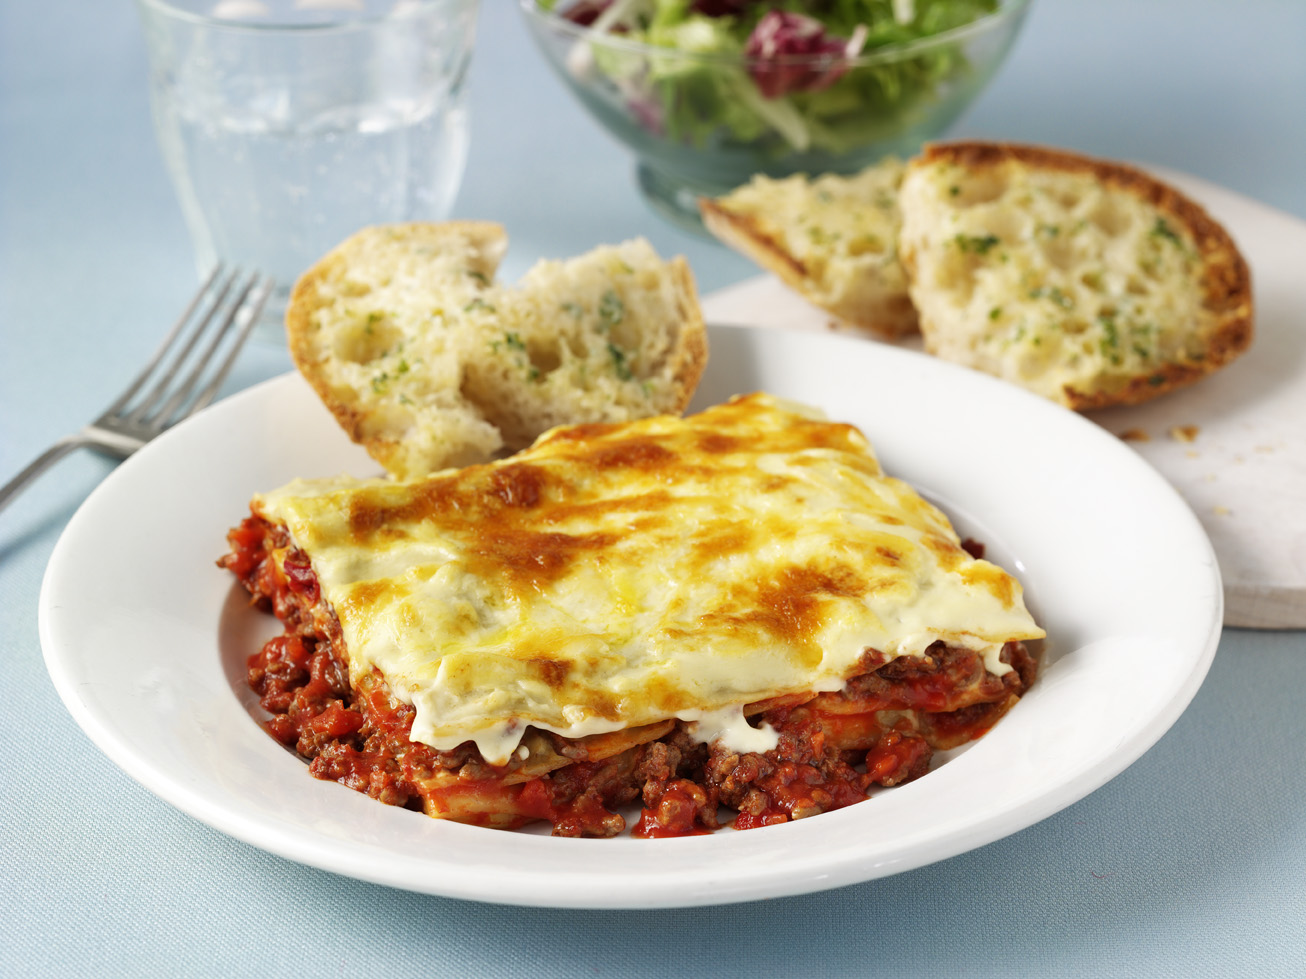
\includegraphics[width=0.65\textwidth]{Lasagne.jpg}
\end{figure}
\newpage

\section*{Lasagne}
% Untertitel
\large{Flei{\ss}arbeit mit Erfolgsgarantie!}
\begin{centering}
% Danach die Zutaten in Tabellenform
% Wie viele werden satt?
F\"{u}r 6 Hungrige
\end{centering}
%\textbf{Zutaten:}
\begin{table}[H]
  \centering
    % eine Tabelle mit insgesamt 4 Spalten, falls mehr Zutaten benoetigt werden
    % links: Menge, rechts: Zutat
  \begin{tabular*}{1\textwidth}{rlrl}
    &\textbf{F\"{u}r das Ragu bolognese:}&&\\
    %&  &&  \\
    1 & M\"{o}hre & 1 Stange & Sellerie \\
    50\,g  & Pancetta & 1 & Zwiebel \\
    2 Zehen & Knoblauch &1\,EL & Butter\\
    1\,EL & Oliven\"{o}l&300\,g&gem. Hackflesich\\
    1 Dose (400\,g)&gesch\"{a}lte Tomaten & 300\,ml& Rotwein/Br\"{u}he\\
    &Salz & & schwarzer Pfeffer\\
    &&&\\

    &\textbf{F\"{u}r die Bechamelsauce:}&&\\
    50\,g & Butter & 50\,g & Mehl \\
    \nicefrac{3}{4}\,l & Milch & & Salz \\
    &schwarzer Pfeffer& & geriebene Muskatnuss\\
    &&&\\
    &\textbf{Zum Einschichten:}&&\\
    250\,g & Nudelplatten & & Salz\\
    250\,g & Mozzarella & 100\,g & frisch geriebener Parmesan\\
    1\,EL & Butter
  \end{tabular*}
\end{table}

%Zubereitung:
\begin{Notes}
  \item F\"{u}r die Bolognese (die genauso gekocht wird, wenn man sie zu
    Spaghetti essen will) M\"{o}hre sch\"{a}len, Sellerie waschen, beides ganz
    fein w\"{u}rfeln. Pancetta ebenfalls in W\"{u}rfelchen schneiden, Zwiebel
    und Knoblauch nach dem Sch\"{a}len auch.

  \item Butter und \"{O}l in der Pfanne oder im Topf warm werden lassen.
    Pancetta, Gem\"{u}se, Zwiebel und Knoblauch dazur\"{u}hren und
    and\"{u}nsten. Hackfleisch untermischen und weitergaren bis es kr\"{u}melig
    ist. Gr\"{o}{\ss}ere Fleischst\"{u}cke dabei mit der R\"{u}ckseite vom
    Kochl\"{o}ffel auseinander dr\"{u}cken, bis sie zerfallen.
    
  \item Tomaten in der Dose klein schneiden, mit dem Wein und der Br\"{u}he
    dazusch\"{u}tten, leict salzen und pfeffern, zugedeckt bei schwacher Hitze 1
    Stunde schmurgeln lassen. Dann erst abschmecken.

  \item Jetzt zur Bechamel: Butter in einem Topf warm werden lasen, braun soll
    sie aber nicht werden. Mit dem Kochl\"{o}ffel flei{\ss}ig r\"{u}hren und das
    Mehl dazusch\"{u}tten. Weiterr\"{u}hren, bis alles glatt ausschaut. Nach und
    nach die Milch dazugie{\ss}en. Jetzt am besten mit dem Schneebesen
    r\"{u}hren, damit sich keine Kl\"{u}mpchen bilden. Sauce 10 Minuten schwach
    k\"{o}cheln lassen, mit Salz, Pfeffer und Muskat w\"{u}rzen.
    
  \item Wer sich f\"{u}r das bisschen Mehrarbeit entschieden hat: 5\,$\ell$
    Wasser mit Salz aufkochen. Nudelplatten darin 4-5\,min kochen, bis sie
    biegsam sind. Mit kaltem Wasser abscherecken.

  \item Mozzarella w\"{u}rfeln. Backofen auf 200\textdegree\,C vorheizen. Eine
    gro{\ss}e rechteckige und feuerfeste Form aus dem Schrank holen. (Die ovale
    nehmen nur Bastelfreaks.) Etwas Bechamel reingie{\ss}en. Nudelplatten drauf,
    Ragu, Bechamel, Mozzarelle und wieder Nudeln. So fortfahren, bis alles in
    der Form ist. Zum Schluss die \"{u}brige Bechamel drauf, mit Parmesan
    bestreuen und mit Butter in Fl\"{o}ckchen belegen. Ab in den Ofen damit.
    Jetzt bleiben 40\,min Zeit zum K\"{u}che aufr\"{a}umen, Tischdecken und
    Ausruhen.

\end{Notes}
So viel Zeit muss sein: gut 2 Stunden, davon 40 Minuten ganz relaxed \newline
Das schmeckt dazu: Rotwein und viel Salat
Pro Portion: 720\,kcal
\vfill
\begin{figure}[H]
  \centering
  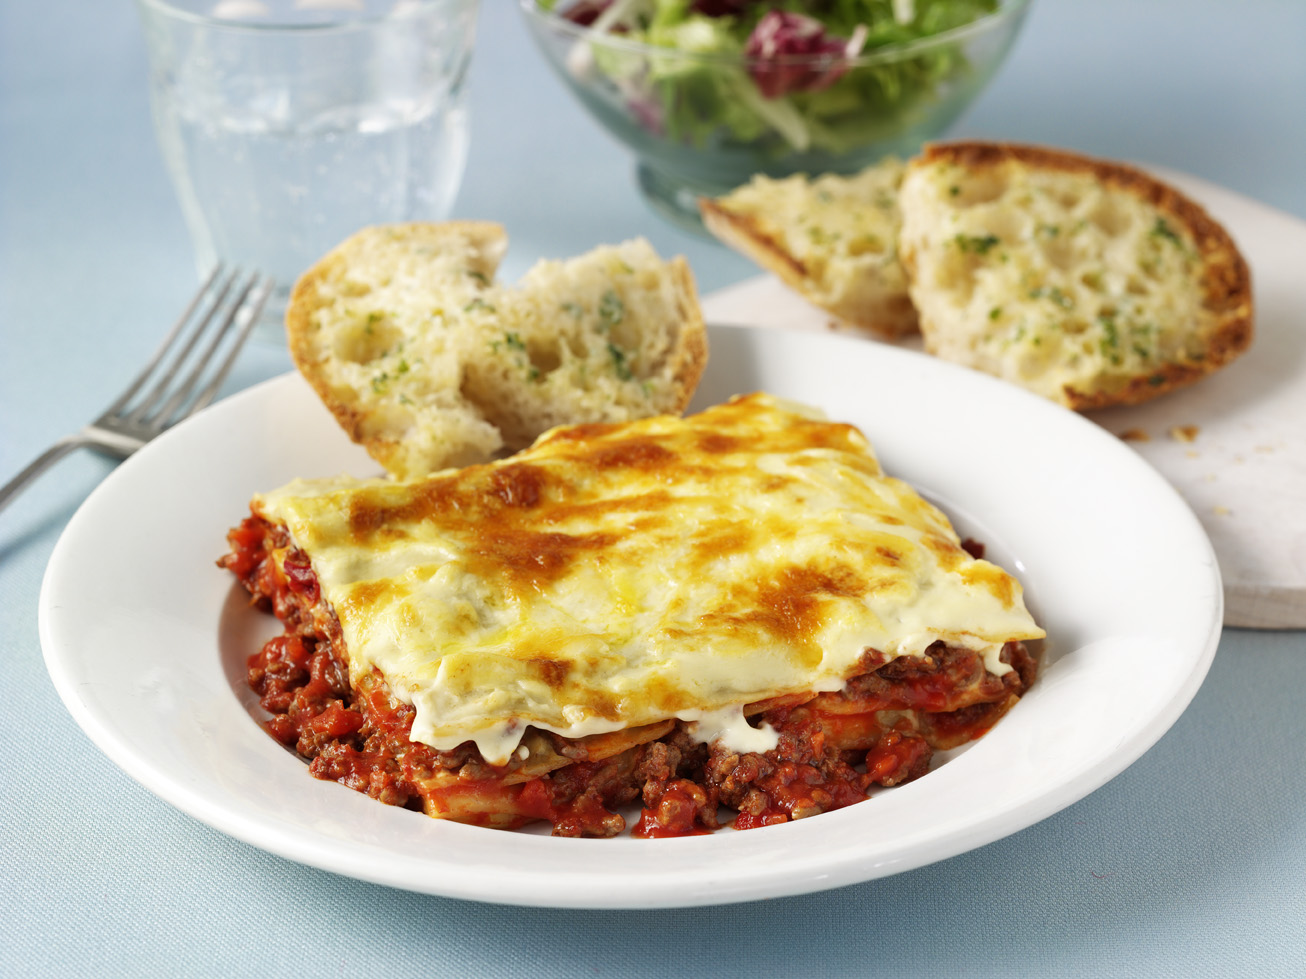
\includegraphics[width=0.65\textwidth]{Lasagne.jpg}
\end{figure}
\newpage
